\documentclass[border=10pt]{standalone}
\usepackage{pgfplots}
\pgfplotsset{compat=1.18}
\definecolor{steelblue}{rgb}{0.27,0.51,0.71}
\begin{document}
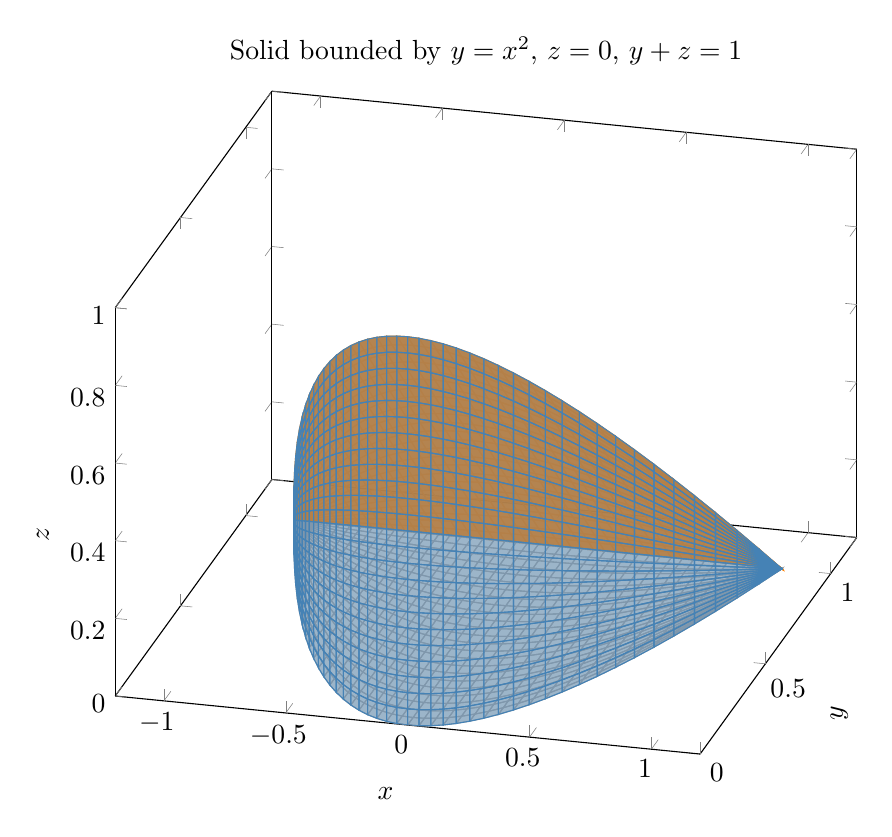
\begin{tikzpicture}
\begin{axis}[
  view={15}{30},
  width=11cm, height=10cm,
  xlabel={$x$}, ylabel={$y$}, zlabel={$z$},
  xmin=-1.2, xmax=1.2, ymin=0, ymax=1.2, zmin=0, zmax=1,
  title={Solid bounded by $y=x^2$, $z=0$, $y+z=1$},
  samples=45, samples y=25,
  domain=-1:1, y domain=0:1,
  axis lines=box,
]
\addplot3[surf, shader=flat, color=orange, fill opacity=0.95]
  ({x}, {x^2+(1-x^2)*y}, {(1-x^2)*(1-y)});
\addplot3[surf, shader=flat, color=gray!70, fill opacity=0.45]
  ({x}, {x^2+(1-x^2)*y}, {0});
\addplot3[surf, shader=flat, color=steelblue, fill opacity=0.4]
  ({x}, {x^2}, {y*(1-x^2)});
\end{axis}
\end{tikzpicture}
\end{document}
